%%%%%%%%%%%%%%%%%%%%%%%%%%%%%%%%%
% modify, as needed
% $ sudo mousepad /usr/local/share/texmf/tex/latex/moderncv/moderncv.cls
% $ sudo latexilla /usr/local/share/texmf/tex/latex/moderncv/moderncv.cls

% XeTex ==> PDF

% use XeTex ==> PDF(Latexmk) 

% 1) xelatex <name_of_tex_file>
% 2) biber <name_of_tex_file>
% 3) xelatex <name_of_tex_file> x 2 
% 
% Weird ==> text runs off first page. Handle w/ \pagebreak but WATCH PLACEMENT of this command or page numbering goes wonky
% A supplemental command that almost worked ==> %\restoregeometry
%%%%%%%%%%%%%%%%%%%%%%%%%%%%%%%



\documentclass[11 pt,letterpaper]{moderncv}        % possible options include font size ('10pt', '11pt' and '12pt'), paper size
                                                   % ('a4paper', 'letterpaper', 'a5paper', 'legalpaper', 'executivepaper' 'landscape')
                                                    
%themes/styles
\moderncvstyle{classic}                           % style options are 'casual' 'classic', 'oldstyle' 'banking'
\moderncvcolor{grey}                              % color options 'blue' 'orange', 'green', 'red', 'purple', 'grey' 'black'




%margins
\usepackage[scale=0.92]{geometry}
%\usepackage[left=0.5in, right=0.5in, top=0.5in, bottom=0.5in]{geometry}
%\usepackage[margin=0.5in]{geometry}

                                                                                               

                               

% fonts                                             % character encoding
\renewcommand{\familydefault}{\rmdefault}         % to set the default font; use '\sfdefault' for the default sans serif font,
%\renewcommand{\familydefault}{newcent}            % '\rmdefault' for the default roman one, or any tex font name

\usepackage[utf8]{inputenc}                       % if you are not using xelatex ou lualatex, replace by the encoding you are using
\usepackage[T1]{fontenc}                           % Use 8-bit encoding that has 256 glyphs



% graphics
\usepackage{tikz}  



% colors
% (in moderncsv.cls)                                        




% headers and footers
% (in moderncsv.cls)  



% bibliography
\usepackage[english]{babel} 
%\usepackage[american]{babel} 
\usepackage[style=verbose,
            sorting=nyt,
            backref=true,           
            doi=false,
            isbn=false,
            url=false,
            backend=biber]{biblatex}
\addbibresource{/home/bruce/Desktop/BibLatex/My_Library_20170125.bib} % BibTeX bibliography file
%\defbibheading{bibempty}{}
%\DeclareLanguageMapping{american}{american-apa}    % avoid yearmonthday problems

% \autocite{ABC01}      %for et al.
% \parencite{}
% \textcite{}            % Shields (2000) ...
% \footcite{}


% footnotes
\usepackage[hang,flushmargin,multiple]{footmisc} 




% footnote help (if needed)
%\makeatletter
%  \deffootnotemark{\textsuperscript{\thefootnotemark}}
%  \long\def\@makefntext#1{\leavevmode\quad(\@thefnmark)~\nobreak\relax#1}
% \makeatother


% pdf
\usepackage{pdfpages}
% example: \includepdf[pages={1-10}]{Experiment1b.pdf}



% watermarks
%\usepackage{everypage} % Required for watermarks
%\usepackage{draftwatermark}
%\SetWatermarkLightness{0.95}
%\SetWatermarkScale{1}




% specialty commands
\newenvironment{myindentpar}[1]%
   {\begin{list}{}%
       {\setlength{\leftmargin}{#1}}%
           \item[]%
   }
     {\end{list}}

%	example:
%\begin{myindentpar}{1em}
%text
%\end{myindentpar}


% misc
\usepackage{ragged2e}
\usepackage{csquotes}
\usepackage{enumitem}


%\nopagenumbers{}                                  % uncomment to suppress automatic page numbering for CVs longer than one page
%\setlength{\hintscolumnwidth}{3cm}                % if you want to change the width of the column with the dates
%\setlength{\makecvtitlenamewidth}{10cm}           % for the 'classic' style, if you want to force the width allocated to your name and
                                                   % avoid line breaks. be careful though, the length is normally calculated to avoid
                                                   % any overlap with your personal info; use this at your own typographical risks...

%\makeatletter
%\renewcommand*{\bibliographyitemlabel}{\@biblabel{\arabic{enumiv}}}
%\makeatother
%\renewcommand*{\bibliographyitemlabel}{[\arabic{enumiv}]}% CONSIDER REPLACING THE ABOVE BY THIS

                                                    % bibliography with mutiple entries
%\usepackage{multibib}
%\newcites{book,misc}{{Books},{Others}}




%----------------------------------------------------------------------------------
%            Contact Info
% ------------------------------------------------------------------------------------
                                                    % personal data
\name{Bruce D.}{Marron}
%\title{Resumé title}                               % optional, remove / comment the line if not wanted
\address{Vito Alessio Robles 237, CP 01050}{}      % optional, remove / comment the line if not wanted; the "postcode city" and
\phone[mobile]{55 4190 9628}                        % optional, remove / comment the line if not wanted
%\phone[fixed]{(503)~236~8483}                        % optional, remove / comment the line if not wanted
%\phone[fax]{+3~(456)~789~012}                         % optional, remove / comment the line if not wanted
\email{marron.bruce.mx@gmail.com}                               % optional, remove / comment the line if not wanted
%\homepage{www.linkedin.com/in/bruce-marron-05496191}                         % optional, remove / comment the line if not wanted
%\extrainfo{}                                          % optional, remove / comment the line if not wanted
%\photo[64pt][0.4pt]{picture}                       % optional, remove / comment the line if not wanted; '64pt' is the height the picture
                                                   % must be resized to, 0.4pt is the thickness of the frame around it (put it to 0pt
                                                   % for no frame) and 'picture' is the name of the picture file
%\quote{Some quote}                                 % optional, remove / comment the line if not wanted



%----------------------------------------------------------------------------------
%          BEGIN DOCUMENT
% ----------------------------------------------------------------------------------
\begin{document}

%---------------------------------------------------
%        RECIPIENT INFO 
%---------------------------------------------------
\recipient{Rectoria}{
MVS Music Centers\\
CDMX}
\date{\today}

%\closing{}
%\enclosure[Attached]{curriculum vit\ae{}}          % use an optional argument to use a string other than "Enclosure", or redefine \enclname

% ---------------------------------------------------
%       BEGIN LETTER
%----------------------------------------------------
\opening{\begin{center}
\vspace{-1.3 cm}
\small{\textbf{RE: Instructor de Guitarra}}
\end{center}
Estimados:}

\makelettertitle
\justifying

%%% START LETTER
\noindent El motivo de la presente carta es para externar que me encuentro altamente interesado en  MVS Music Centers y me motiva conocer que UTECA colabora de manera significatica con ustedes. Durante este cuatrimestre estaré cumpliendo un año trabajando como profesor en UTECA, dando clases en terminología (ciencias, jurídica, economía) e inglés avanzado. Pero mi alma y una de mis principales pasiones siempre será la música, y me encantaría extender mi servicio a MVS Music Centers dando clases de guitarra.

\noindent Siempre me he involucrado en los \textit{Arts and Sciences}. Empecé con la guitarra a los 12 años y tuve oportunidades de estudiar a nivel universitario y tocar como profesional. Llevo 36 créditos universitarios en teoría musical, entrenamiento auditivo, piano básico, historia de música, bandas de jazz, e improvisación. He estudiado guitarra clásica con Michael Chapdelaine, maestro de guitarra clásica y \textit{fingerpicking} y el único guitarrista apremiado \textit{First Place} en dos géneros: ganó el \textit{Guitar Foundation of America International Classical Guitar Competition} y también el \textit{National Fingerstyle Championships at the Walnut Valley Bluegrass Festival}. He estudiado guitarra jazz con Michael Anthony, un \textit{session player} (estudiante de Howard Roberts) que fue el \textit{first call} guitarrista en Los Angeles, California durante los 70s.

\noindent En Albuquerque, New Mexico tuve mi propia escuela de guitarra. He trabajado profesionalmente contratado por guitarrista de orquesta en musicales (\textit{The Sound of Music, Godspell, Camelot, and Fiddler on the Roof}) y en varios conjuntos musicales. Algunas de mis fortalezas son el canto y el trabajo en equipo en la participación como miembro de bandas y proyectos diversos. En 2023 fundé MOZ Espectaculos, dando como resultado un show en Foro Coyocanense con obras originales y covers.


Considero cuento con las habilidades, herramientas y motivación para ser un gran elemento en su equipo, podría desempeñarme de manera  excelente para los alumnos principiantes de guitarra en MVS Music Centers por los siguentes razones:
\begin{itemize}
  \item \textbf{Base Integral} -- La guitarra es un instrumento difícil de dominar para el estudiante serio o aún un aficionado. En todos los casos, puedo dar los estudiantes bases firmes e integrales (teoría, tecnicas, conceptos, ejercicios) para tener confianza y lograr sus metas.
  \item \textbf{Diversidad y Musicalidad} -- Puedo introducir estilos diversos para desarrollar flexibilidad y musicalidad en el instrumento.
  \item \textbf{Experiencia} -- Tocando en la casa y tocando en el escenario son cosas muy distintas. Para los estudientes que quisieran tocar en público, puedo brindarles consejos y métodos de preparación.
\end{itemize}
Al fin de cuentas, me gusta mucho la profesion de la docencia, sea en escuelas públicas, universidades, o salones de música. También cuento con un bagaje amplio de materiales, conocimientos y experiencias para generar un curriculum que nutra de manera integral a todos los estudiantes.

Agradezco la atencion y consideracion. Esperando poder colaborar en conjunto y difundir el conocimiento musical más allá de las aulas.

Sinceramente,

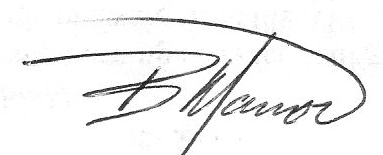
\includegraphics[scale=.65]{graphics/signature.jpeg}\\
Bruce D. Marron \\
Coyoacán, CDMX

\end{document}
